\chapter{Experiment: hardware system}
In this chapter, we discuss experiments conducted on the hardware system. The content is organized into four sections. The first section provides an overview of the hardware setup for the double pendulum system. The second section delves into the system identification of the hardware. The third section details our approach to addressing the sim-to-real gap challenge. The final section presents the successful outcomes of our hardware experiments.

\section{Hardware setup}
Mechanically, the double pendulum system is a straightforward 2-R linkage. The first revolute joint attaches to the base, while the second one connects the two links. Quasi-direct drive motors are mounted on each joint to provide torque, and a counterweight is positioned at the end of the second link.

Our mechanical design for the double pendulum underwent two iterations. In the initial design, the base consisted of a bent aluminum plate, and the links featured a sandwich structure with aluminum on the outside and engineering plastic on the inside. These links were of homogeneous size, meaning that the cross-sectional areas at the link intersections were consistent. We abandoned this design due to rotational imbalances. Specifically, the rotation plane of the links wasn't consistently perpendicular to the motor axes, leading to vibrations and accelerated wear during regular use. In extreme cases, when the links rotated at high angular velocities, this imbalance was exacerbated. This not only resulted in the links bending but also led to catastrophic system failures. Such failures presented significant safety risks to personnel.

In the second iteration, we addressed the issues encountered in the previous design, leading to two major modifications. First, we replaced the aluminum-plastic combination with a carbon fiber-foam blend. While the incorporation of carbon fiber marginally increased the cost, it significantly boosted the yield strength. Second, we introduced triangular-shaped links with central cutouts. This design, while lightweight, also substantially enhanced the yield strength due to the changed intersections. Overall, this iteration resulted in a mechanical structure that is considerably more reliable than the first.
\begin{figure}[htbp]
\begin{minipage}[b]{0.45\linewidth}
\centering
\fbox{\includegraphics[width=0.75\linewidth]{figures/double_pendulum_CAD.png}}
\end{minipage}
% Example to add your own logos for Acknowledgment
%\hfill
\begin{minipage}[b]{0.45\linewidth}
\centering
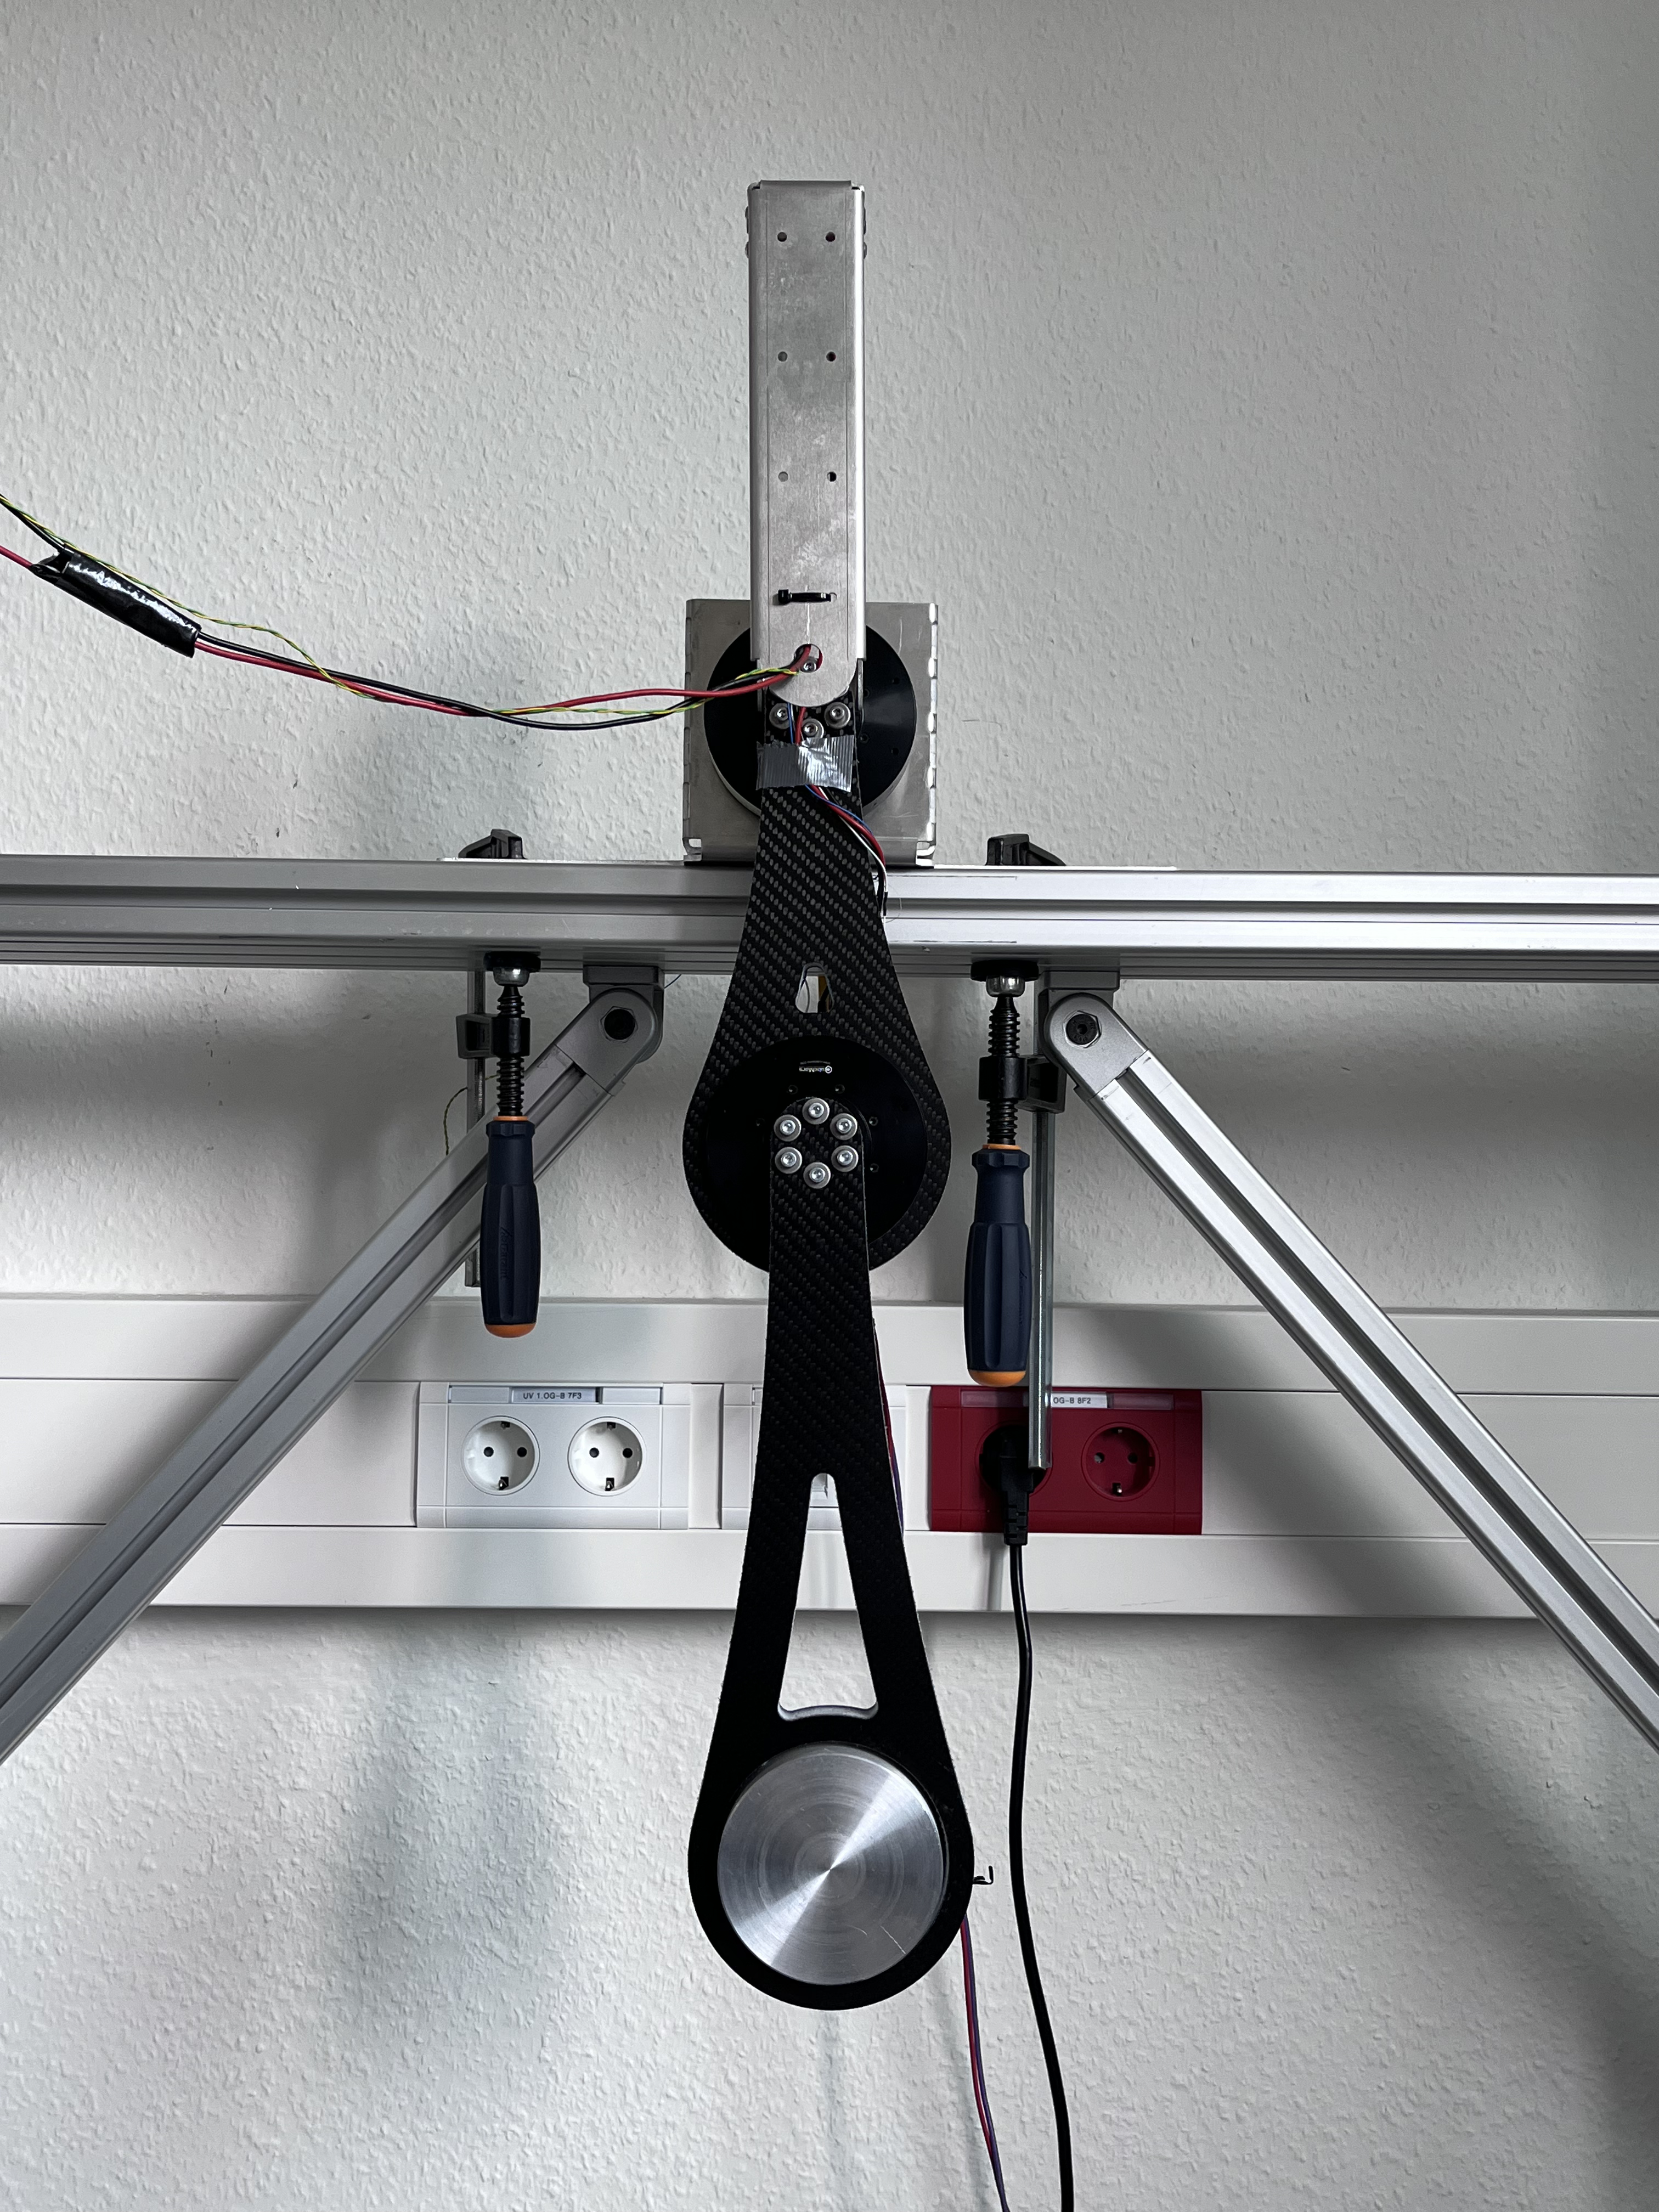
\includegraphics[width=1.0\linewidth]{figures/double_pendulum_real_system.png}
\end{minipage}
\caption{Double pendulum setup in CAD and in real world}
\end{figure}

For the quasi-direct drive motors, we selected the AK80-6 V100 model from the company CubeMars. This motor's design facilitates easy mounting from both the front and rear ends. As depicted in Figure5.2(b), the motor's maximum torque during continuous operation is 6 Nm, which aligns well with our torque limit of 5 Nm. Additionally, the motor is designed for compatibility with both serial bus and CAN bus, simplifying the development process.


\begin{figure}[htbp]
  \centering
  \begin{subfigure}[b]{0.45\textwidth}
    \centering
    \includegraphics[width=\textwidth]{figures/hardware_setup/motor.jpg}
    \caption{Figure A}
    \label{fig:subfiga}
  \end{subfigure}
  \hfill
  \begin{subfigure}[b]{0.45\textwidth}
    \centering
    \includegraphics[width=\textwidth]{figures/hardware_setup/torque_speed_curve.jpg}
    \label{fig:subfigb}
    \caption{Figure B}
  \end{subfigure}
  \caption{Two figures side by side}
  \label{fig:twosubfigures}
\end{figure}

\section{System identification}
This section is about the system identification problem when using hardware system.

\section{Sim2real problem}
This section is about sim2real problem.

\begin{figure}[htbp]
    \centering
    \fbox{\includegraphics[width=0.9\textwidth]{figures/hardware_result/pendubot_noisy_unclipped.png}} % Second image
    \caption{pendubot noisy simulation result}
    \label{fig:image_b}
\end{figure}






\section{Real hardware results}
This section is about simulation results in pendubot and acrobot.

\subsection{pendubot results}
pendubot:

\subsection{acrobot results}
acrobot:

\cleardoublepage
